\documentclass[12pt, a4paper, oneside]{ctexart}
\usepackage{amsmath, amsthm, amssymb, bm, color, graphicx, geometry, mathrsfs,extarrows, braket, booktabs, array, wrapfig, enumitem, subfigure, bbm}
\usepackage[colorlinks,linkcolor=red,anchorcolor=blue,citecolor=blue,urlcolor=blue,menucolor=black]{hyperref}
%%%% 设置中文字体 %%%%
% fc-list -f "%{family}\n" :lang=zh >d:zhfont.txt 命令查看已有字体
\setCJKmainfont{方正书宋.ttf}[BoldFont = 方正黑体_GBK.ttf, ItalicFont = simkai.ttf, BoldItalicFont = 方正粗楷简体.ttf]
%%%% 设置英文字体 %%%%
\setmainfont{Times New Roman}
\setsansfont{Calibri}
\setmonofont{Consolas}

%%%% 设置代码块 %%%%
% 在vscode中使用minted需要先配置python解释器, Ctrl+Shift+P, 输入Python: Select Interpreter选择安装了Pygments的Python版本. 再在setting.json中xelatex和pdflatex的参数中加入 "--shell-escape", 即可
% TeXworks中配置方法参考: https://blog.csdn.net/RobertChenGuangzhi/article/details/108140093
\usepackage{minted}
\renewcommand{\theFancyVerbLine}{
    \sffamily\textcolor[rgb]{0.5,0.5,0.5}{\scriptsize\arabic{FancyVerbLine}}} % 修改代码前序号大小
% 加入不同语言的代码块
\newmintinline{cpp}{fontsize=\small, linenos, breaklines, frame=lines}
\newminted{cpp}{fontsize=\small, baselinestretch=1, linenos, breaklines, frame=lines}
\newmintedfile{cpp}{fontsize=\small, baselinestretch=1, linenos, breaklines, frame=lines}
\newmintinline{matlab}{fontsize=\small, linenos, breaklines, frame=lines}
\newminted{matlab}{fontsize=\small, baselinestretch=1, mathescape, linenos, breaklines, frame=lines}
\newmintedfile{matlab}{fontsize=\small, baselinestretch=1, linenos, breaklines, frame=lines}
\newmintinline{python}{fontsize=\small, linenos, breaklines, frame=lines, python3}  % 使用\pythoninline{代码}
\newminted{python}{fontsize=\small, baselinestretch=1, linenos, breaklines, frame=lines, python3}  % 使用\begin{pythoncode}代码\end{pythoncode}
\newmintedfile{python}{fontsize=\small, baselinestretch=1, linenos, breaklines, frame=lines, python3}  % 使用\pythonfile{代码地址}

%%%% 设置行间距与页边距 %%%%
\linespread{1.4}
%\geometry{left=2.54cm,right=2.54cm,top=3.18cm,bottom=3.18cm}
\geometry{left=1.84cm,right=1.84cm,top=2.18cm,bottom=2.18cm}

%%%% 图片相对路径 %%%%
\graphicspath{{figures/}} % 当前目录下的figures文件夹, {../figures/}则是父目录的figures文件夹
\setlength{\abovecaptionskip}{-0.2cm}  % 缩紧图片标题与图片之间的距离
\setlength{\belowcaptionskip}{0pt} 

%%%% 缩小item,enumerate,description两行间间距 %%%%
\setenumerate[1]{itemsep=0pt,partopsep=0pt,parsep=\parskip,topsep=5pt}
\setitemize[1]{itemsep=0pt,partopsep=0pt,parsep=\parskip,topsep=5pt}
\setdescription{itemsep=0pt,partopsep=0pt,parsep=\parskip,topsep=5pt}

%%%% 自定义公式 %%%%
\everymath{\displaystyle} % 默认全部行间公式
\DeclareMathOperator*\uplim{\overline{lim}} % 定义上极限 \uplim_{}
\DeclareMathOperator*\lowlim{\underline{lim}} % 定义下极限 \lowlim_{}
\DeclareMathOperator*{\argmax}{arg\,max}  % 定义取最大值的参数 \argmax_{}
\DeclareMathOperator*{\argmin}{arg\,min}  % 定义取最小值的参数 \argmin_{}
\let\leq=\leqslant % 将全部leq变为leqslant
\let\geq=\geqslant % geq同理
\DeclareRobustCommand{\rchi}{{\mathpalette\irchi\relax}}
\newcommand{\irchi}[2]{\raisebox{\depth}{$#1\chi$}} % 使用\rchi将\chi居中

%%%% 自定义环境配置 %%%%
\newcounter{problem}  % 问题序号计数器
\newenvironment{problem}[1][]{\stepcounter{problem}\par\noindent\textbf{题目\arabic{problem}. #1}}{\smallskip\par}
\newenvironment{solution}[1][]{\par\noindent\textbf{#1解答. }}{\smallskip\par}  % 可带一个参数表示题号\begin{solution}{题号}
\newenvironment{note}{\par\noindent\textbf{注记. }}{\smallskip\par}
\newenvironment{remark}{\begin{enumerate}[label=\textbf{注\arabic*.}]}{\end{enumerate}}
\BeforeBeginEnvironment{minted}{\vspace{-0.5cm}}  % 缩小minted环境距上文间距
\AfterEndEnvironment{minted}{\vspace{-0.2cm}}  % 缩小minted环境距下文间距

%%%% 一些宏定义 %%%%
\def\bd{\boldsymbol}        % 加粗(向量) boldsymbol
\def\disp{\displaystyle}    % 使用行间公式 displaystyle(默认)
\def\weekto{\rightharpoonup}% 右半箭头
\def\tsty{\textstyle}       % 使用行内公式 textstyle
\def\sign{\text{sign}}      % sign function
\def\wtd{\widetilde}        % 宽波浪线 widetilde
\def\R{\mathbb{R}}          % Real number
\def\N{\mathbb{N}}          % Natural number
\def\Z{\mathbb{Z}}          % Integer number
\def\Q{\mathbb{Q}}          % Rational number
\def\C{\mathbb{C}}          % Complex number
\def\K{\mathbb{K}}          % Number Field
\def\P{\mathbb{P}}          % Polynomial
\def\1{\mathbbm{1}}
\def\d{\mathrm{d}}          % differential operator
\def\e{\mathrm{e}}          % Euler's number
\def\i{\mathrm{i}}          % imaginary number
\def\re{\mathrm{Re}}        % Real part
\def\im{\mathrm{Im}}        % Imaginary part
\def\res{\mathrm{Res}}      % Residue
\def\ker{\mathrm{Ker}}      % Kernel
\def\vspan{\mathrm{vspan}}  % Span  \span与latex内核代码冲突改为\vspan
\def\L{\mathcal{L}}         % Loss function
\def\O{\mathcal{O}}         % big O notation
\def\wdh{\widehat}          % 宽帽子 widehat
\def\ol{\overline}          % 上横线 overline
\def\ul{\underline}         % 下横线 underline
\def\add{\vspace{1ex}}      % 增加行间距
\def\del{\vspace{-1.5ex}}   % 减少行间距

%%%% 定理类环境的定义 %%%%
\newtheorem{theorem}{定理}

%%%% 基本信息 %%%%
\newcommand{\RQ}{\today} % 日期
\newcommand{\km}{强化学习} % 科目
\newcommand{\bj}{强基数学002} % 班级
\newcommand{\xm}{吴天阳} % 姓名
\newcommand{\xh}{2204210460} % 学号

\begin{document}

%\pagestyle{empty}
\pagestyle{plain}
\vspace*{-15ex}
\centerline{\begin{tabular}{*5{c}}
    \parbox[t]{0.25\linewidth}{\begin{center}\textbf{日期}\\ \large \textcolor{blue}{\RQ}\end{center}} 
    & \parbox[t]{0.2\linewidth}{\begin{center}\textbf{科目}\\ \large \textcolor{blue}{\km}\end{center}}
    & \parbox[t]{0.2\linewidth}{\begin{center}\textbf{班级}\\ \large \textcolor{blue}{\bj}\end{center}}
    & \parbox[t]{0.1\linewidth}{\begin{center}\textbf{姓名}\\ \large \textcolor{blue}{\xm}\end{center}}
    & \parbox[t]{0.15\linewidth}{\begin{center}\textbf{学号}\\ \large \textcolor{blue}{\xh}\end{center}} \\ \hline
\end{tabular}}
\begin{center}
    \zihao{3}\textbf{第四章作业}
\end{center}\vspace{-0.2cm}
\begin{problem}[例4.2(杰克租车问题)]
    Jack管理一家有两个地点A、B的汽车公司,每天会有用户前往一个地点租车,如果租出去一辆车,则可获得$10$美元收益,如果在那个地点没有汽车则无法租出去;
    同时每天还会有人还车,还的车在第二天变得可用. 我们假设每天租车数量和还车数量分别满足期望为$\lambda,\sigma$的Poisson分布$\text{Poi}(\lambda)\sim\frac{\lambda^n}{n!}\e^{-\lambda}$,

    同时Jack还可以在每天晚上将A、B的汽车进行移动,每次移动一辆车代价为$2$美元,并且每天最多移动$5$辆车,且假设一个地点的车辆数目不能超过$20$辆车,额外的车会自动消失.

    我们令折扣率$\gamma = 0.9$,状态为每天结束时每个地点的车辆数目,动作为夜间在两个地点移动的车辆数目.
\end{problem}
\begin{solution}首先用数学符号将状态、动作和收益表示出来:

    \textbf{状态}:设$nA_t, nB_t$分别表示第$t$天结束时$A,B$两地的车辆数目,
    则状态$S_t = (nA_t, nB_t)$. 假设第$t$天$A$地归还的车辆数为$inA_t\sim \text{Poi}(3)$,
    $B$地归还的车辆数为$inB_t\sim \text{Poi}(2)$,于是状态$S_t= (nA_t,nB_t)$满足:
    \begin{align*}
        &\ nA_t = \min\{nA_{t-1}-outA_t+move_t+inA_t, 20\}\\
        &\ nB_t = \min\{nB_{t-1} - outB_t - move_t + inB_t, 20\}
    \end{align*}

    \textbf{动作}:设$move_t\in [-5, 5]$,表示第$t$天晚上移动的车辆,当$move_t > 0$表示从$A$处移出$move_t$辆车到$B$处;
    当$move_t < 0$表示从$B$处移出$-move_t$辆车到$A$处.

    \textbf{收益}:设$A,B$两地第$t$天成功租出的车数量分别为$outA_t = \min(xA, nA_{t-1}), outB_t = \min(xB, nB_{t-1})$,
    其中$xA\sim \text{Poi}(3),xB\sim \text{Poi}(4)$分别表示第$t$天来租车的人数. 则第$t$天的收益为
    \begin{equation*}
        R_t = 10(outA + outB) - 2|move_t|
    \end{equation*}
    通过3次迭代策略达到稳定,第0,1,3次策略和最终的状态价值函数如下图所示:
    %%%% 两组图并排放(可溢出一些) %%%%
    \begin{figure}[htbp]
        \hspace{-2.2cm}
        \subfigure  % 子图的标题
        {
            % 如果一行放三个图改成0.3\linewidth即可
            \begin{minipage}[b]{.6\linewidth}
                \centering
                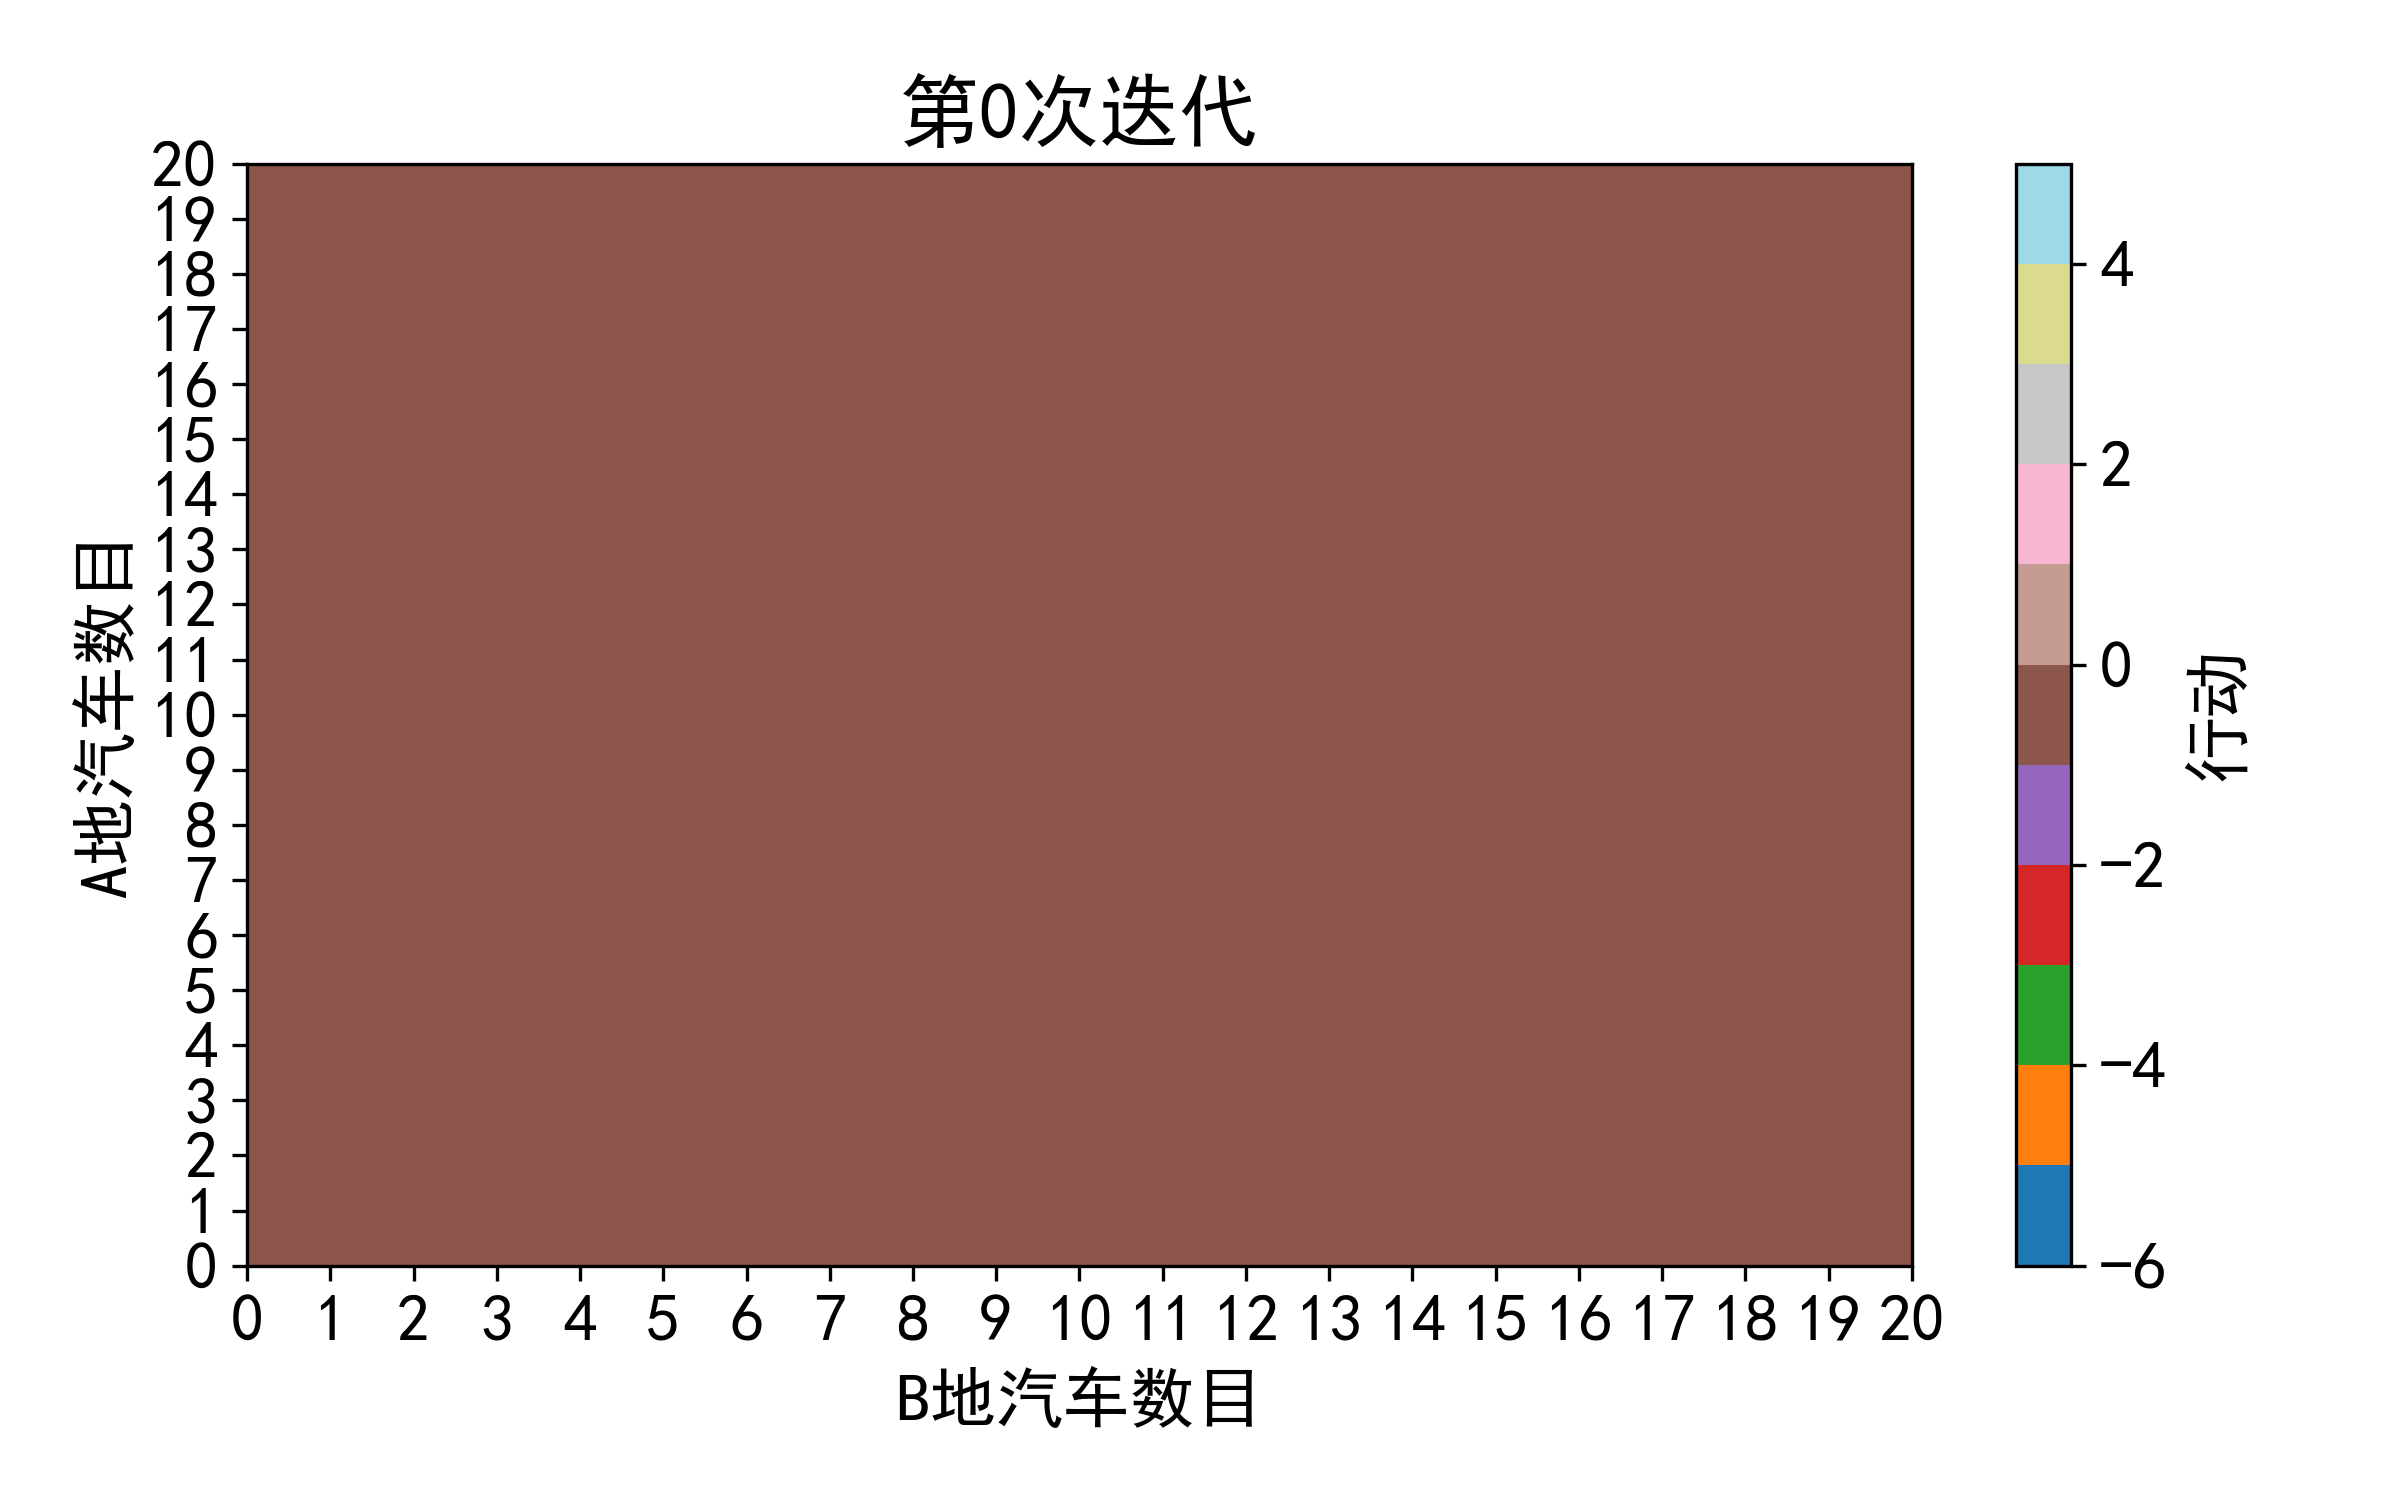
\includegraphics[scale=0.52]{078/078页例题4.2policy0.png}
            \end{minipage}
        }
        \subfigure
        {
            \begin{minipage}[b]{.2\linewidth}
                \centering
                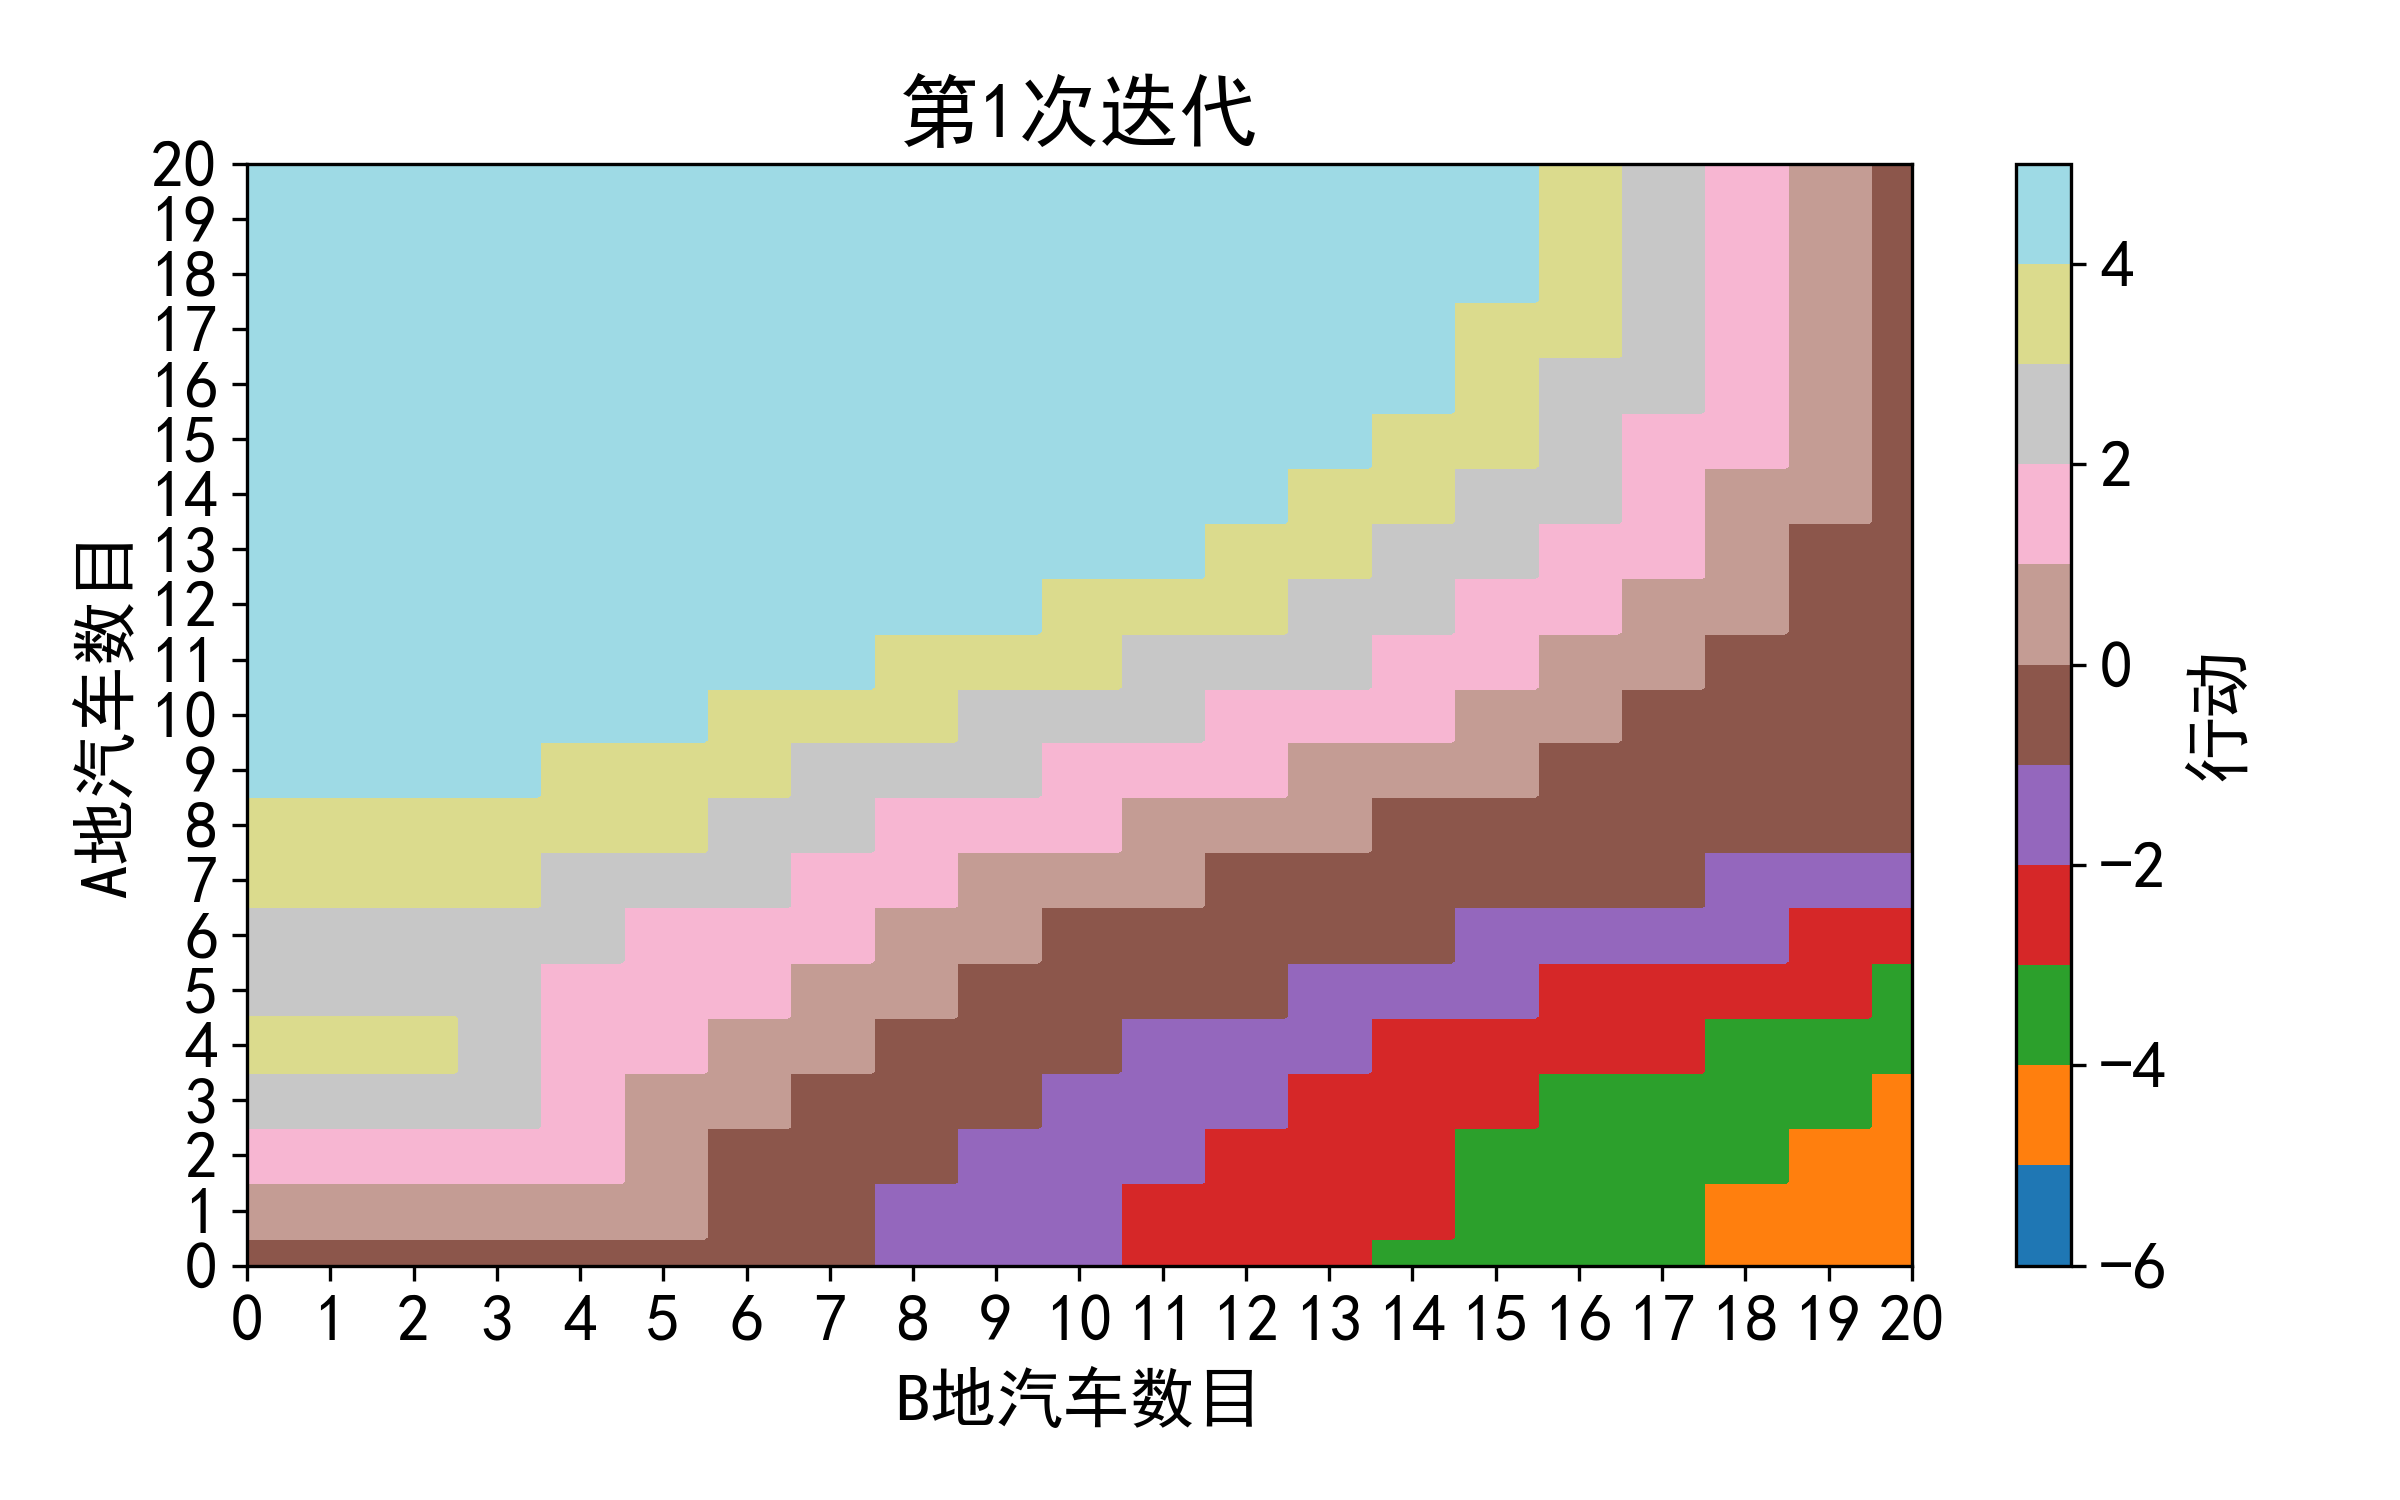
\includegraphics[scale=0.52]{078/078页例题4.2policy1.png}
            \end{minipage}
        }
    \end{figure}
    \begin{figure}[htbp]
        \hspace{-0.5cm}
        \subfigure  % 子图的标题
        {
            % 如果一行放三个图改成0.3\linewidth即可
            \begin{minipage}[b]{.62\linewidth}
                \centering
                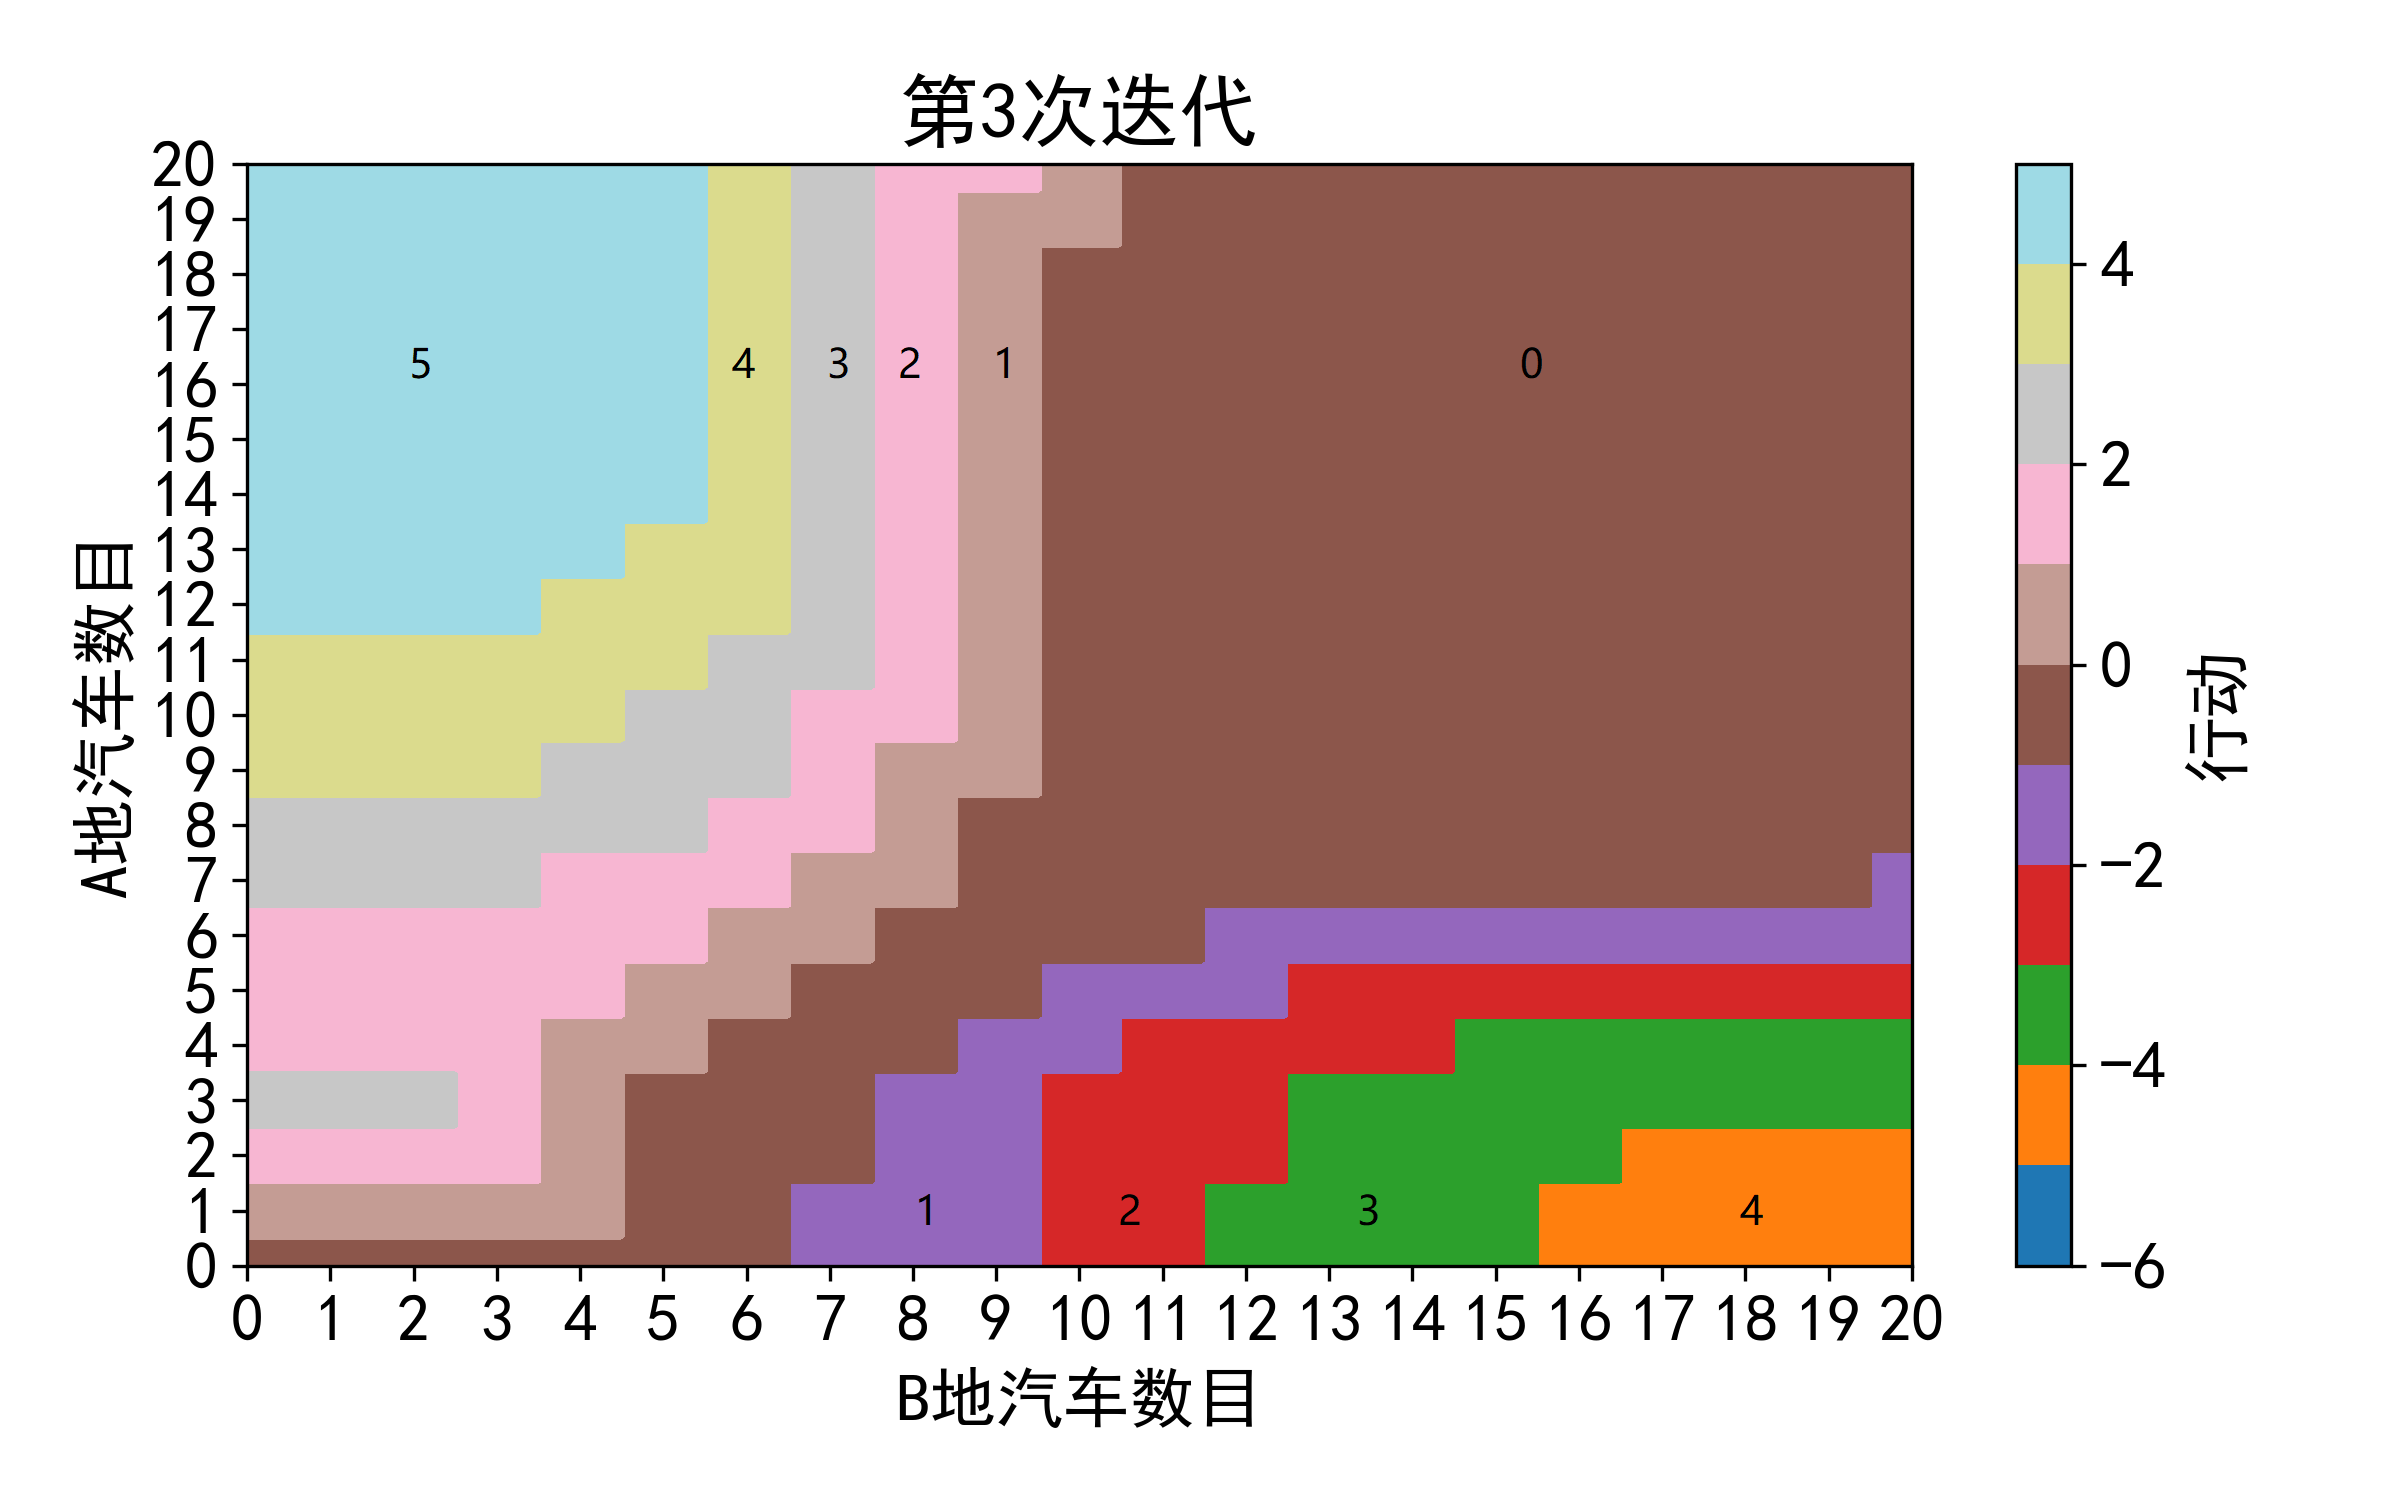
\includegraphics[scale=0.22]{078/078页例题4.2policy3.png}
            \end{minipage}
        }
        \subfigure
        {
            \begin{minipage}[b]{.2\linewidth}
                \centering
                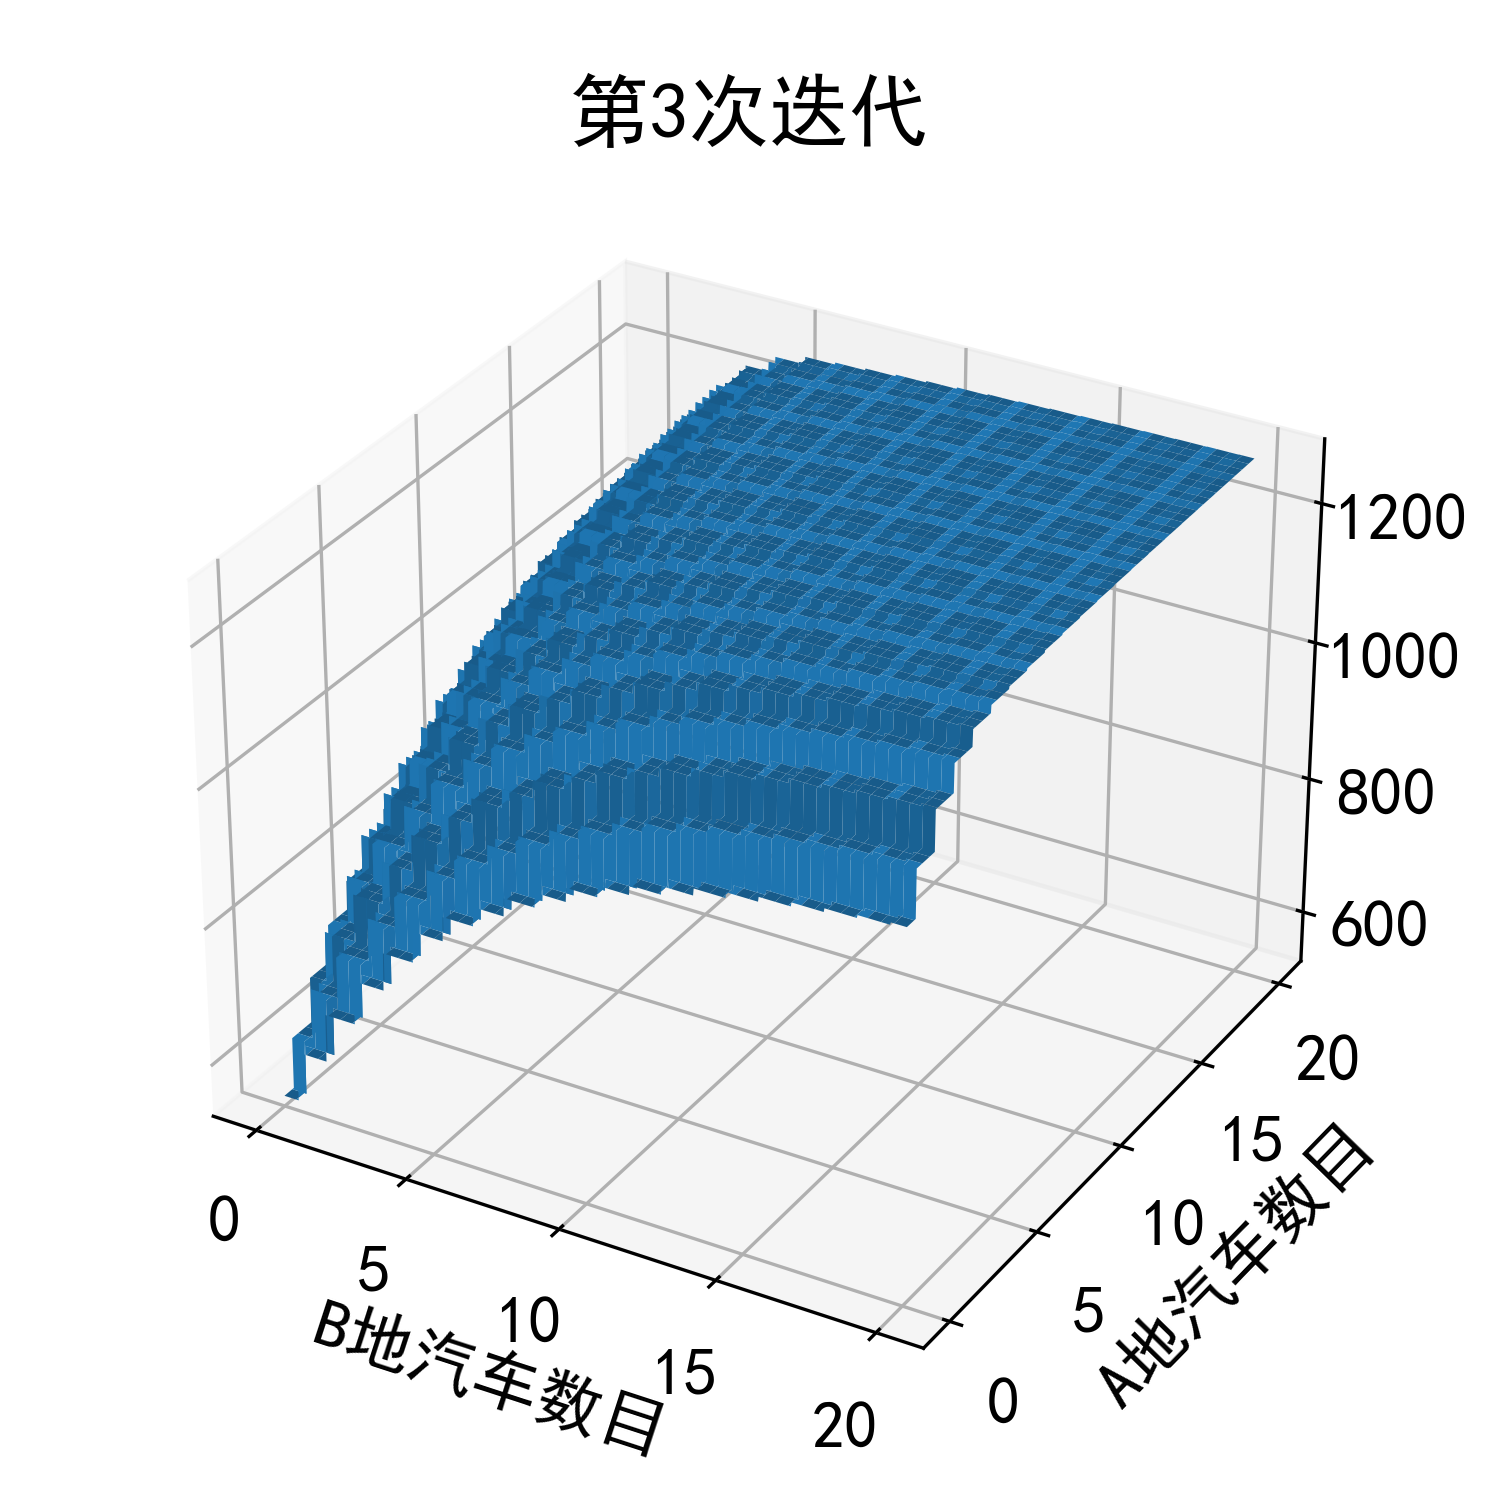
\includegraphics[scale=0.52]{078/078页例题4.2value3.png}
            \end{minipage}
        }
    \end{figure}
\end{solution}
\begin{problem}[练习4.7]
    使用动态规划方法解决以下更改过的Jack租车问题,Jack一个员工在A地点上班,每晚会做公车达到B地点,
    她可以免费将A地点的一辆车移动到B地点,其他车辆的移动仍需要2美元,并且Jack的停车场有限,
    如果在某个地点过夜的车辆数目大于$10$辆,则需要在另一个停车场支付$4$美元(无论多少车)来停车.
\end{problem}
\begin{solution}
    只需对例4.2的基础上对$R_t$稍加修改即可:
    \begin{equation*}
            R_t = \begin{cases}
                10(outA + outB) - 2(move_t - 1) - 4\cdot\1_{nA_t > 10} - 4\cdot\1_{nB_t > 10},&\quad move_t > 0,\\
                10(outA + outB) + 2move_t - 4\cdot\1_{nA_t > 10} - 4\cdot\1_{nB_t > 10},&\quad move_t \leq 0,\\
            \end{cases}
    \end{equation*}
    其中$\1_{nA_t>10}$表示当$nA_t>10$时为$1$,否则为$0$.

    通过4次迭代达到稳定,第1,2,4次策略和最终的状态价值函数如下
    \begin{figure}[htbp]
        \hspace{-2.2cm}
        \subfigure  % 子图的标题
        {
            % 如果一行放三个图改成0.3\linewidth即可
            \begin{minipage}[b]{.6\linewidth}
                \centering
                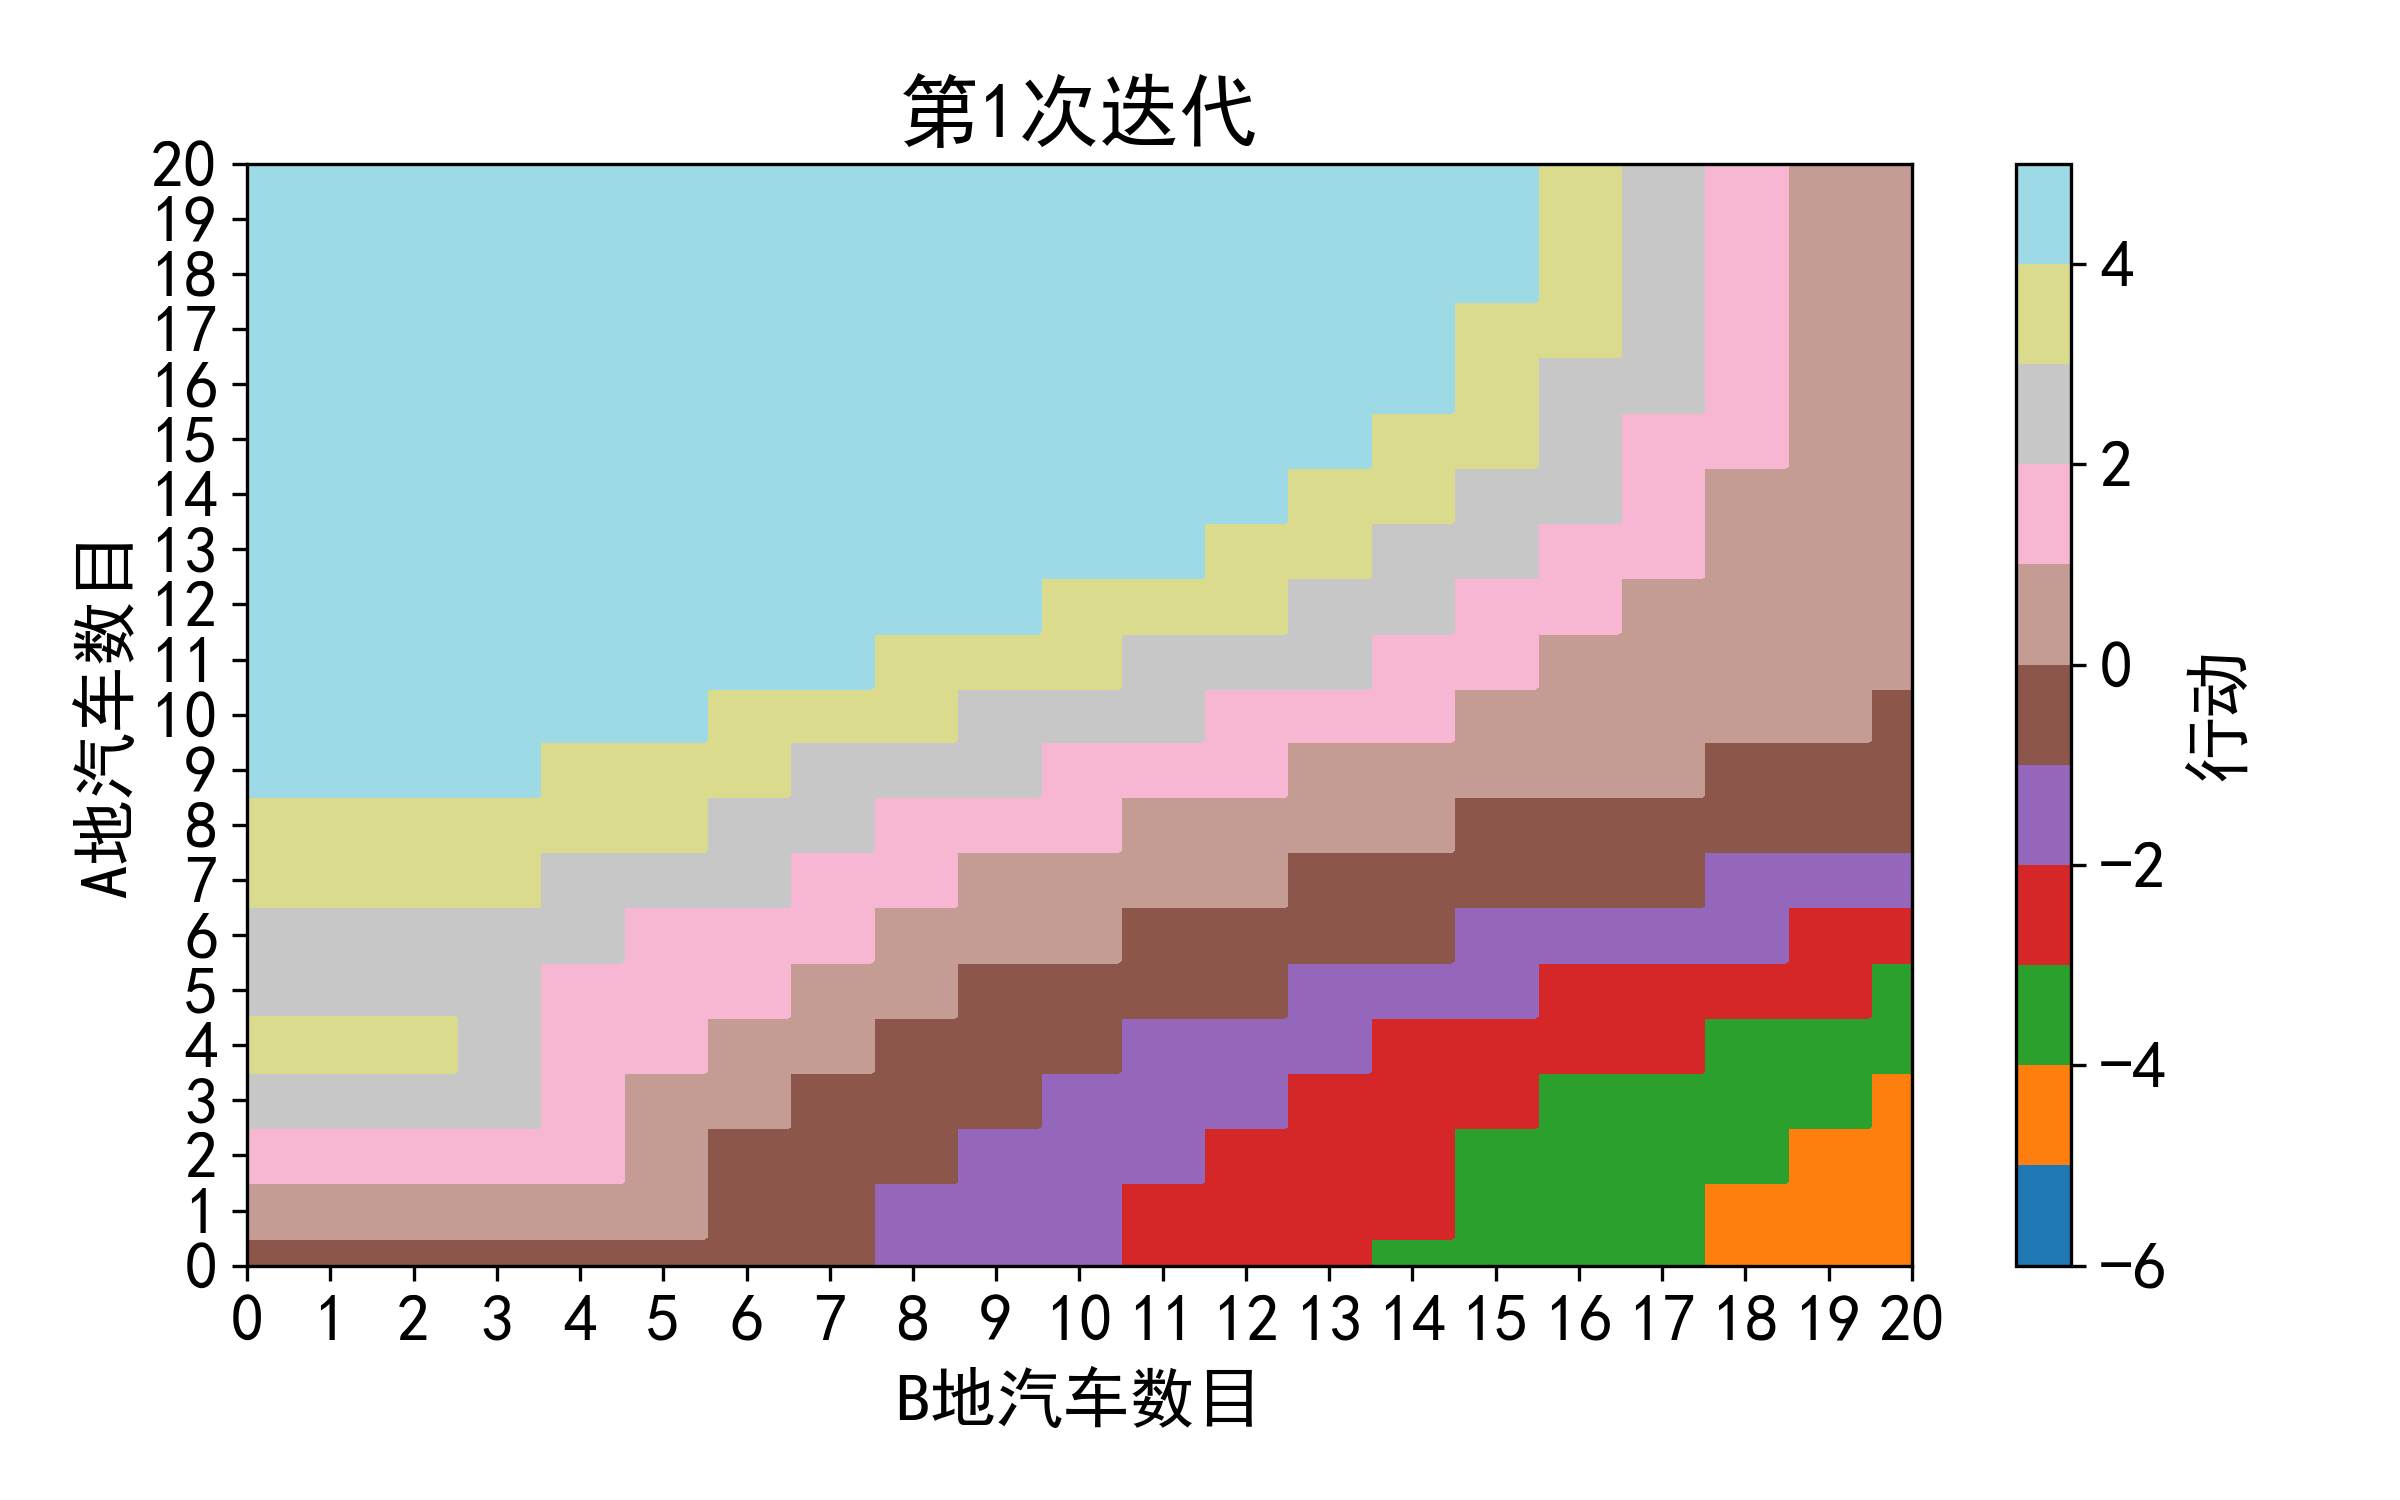
\includegraphics[scale=0.52]{080/080页练习4.7policy1.png}
            \end{minipage}
        }
        \subfigure
        {
            \begin{minipage}[b]{.2\linewidth}
                \centering
                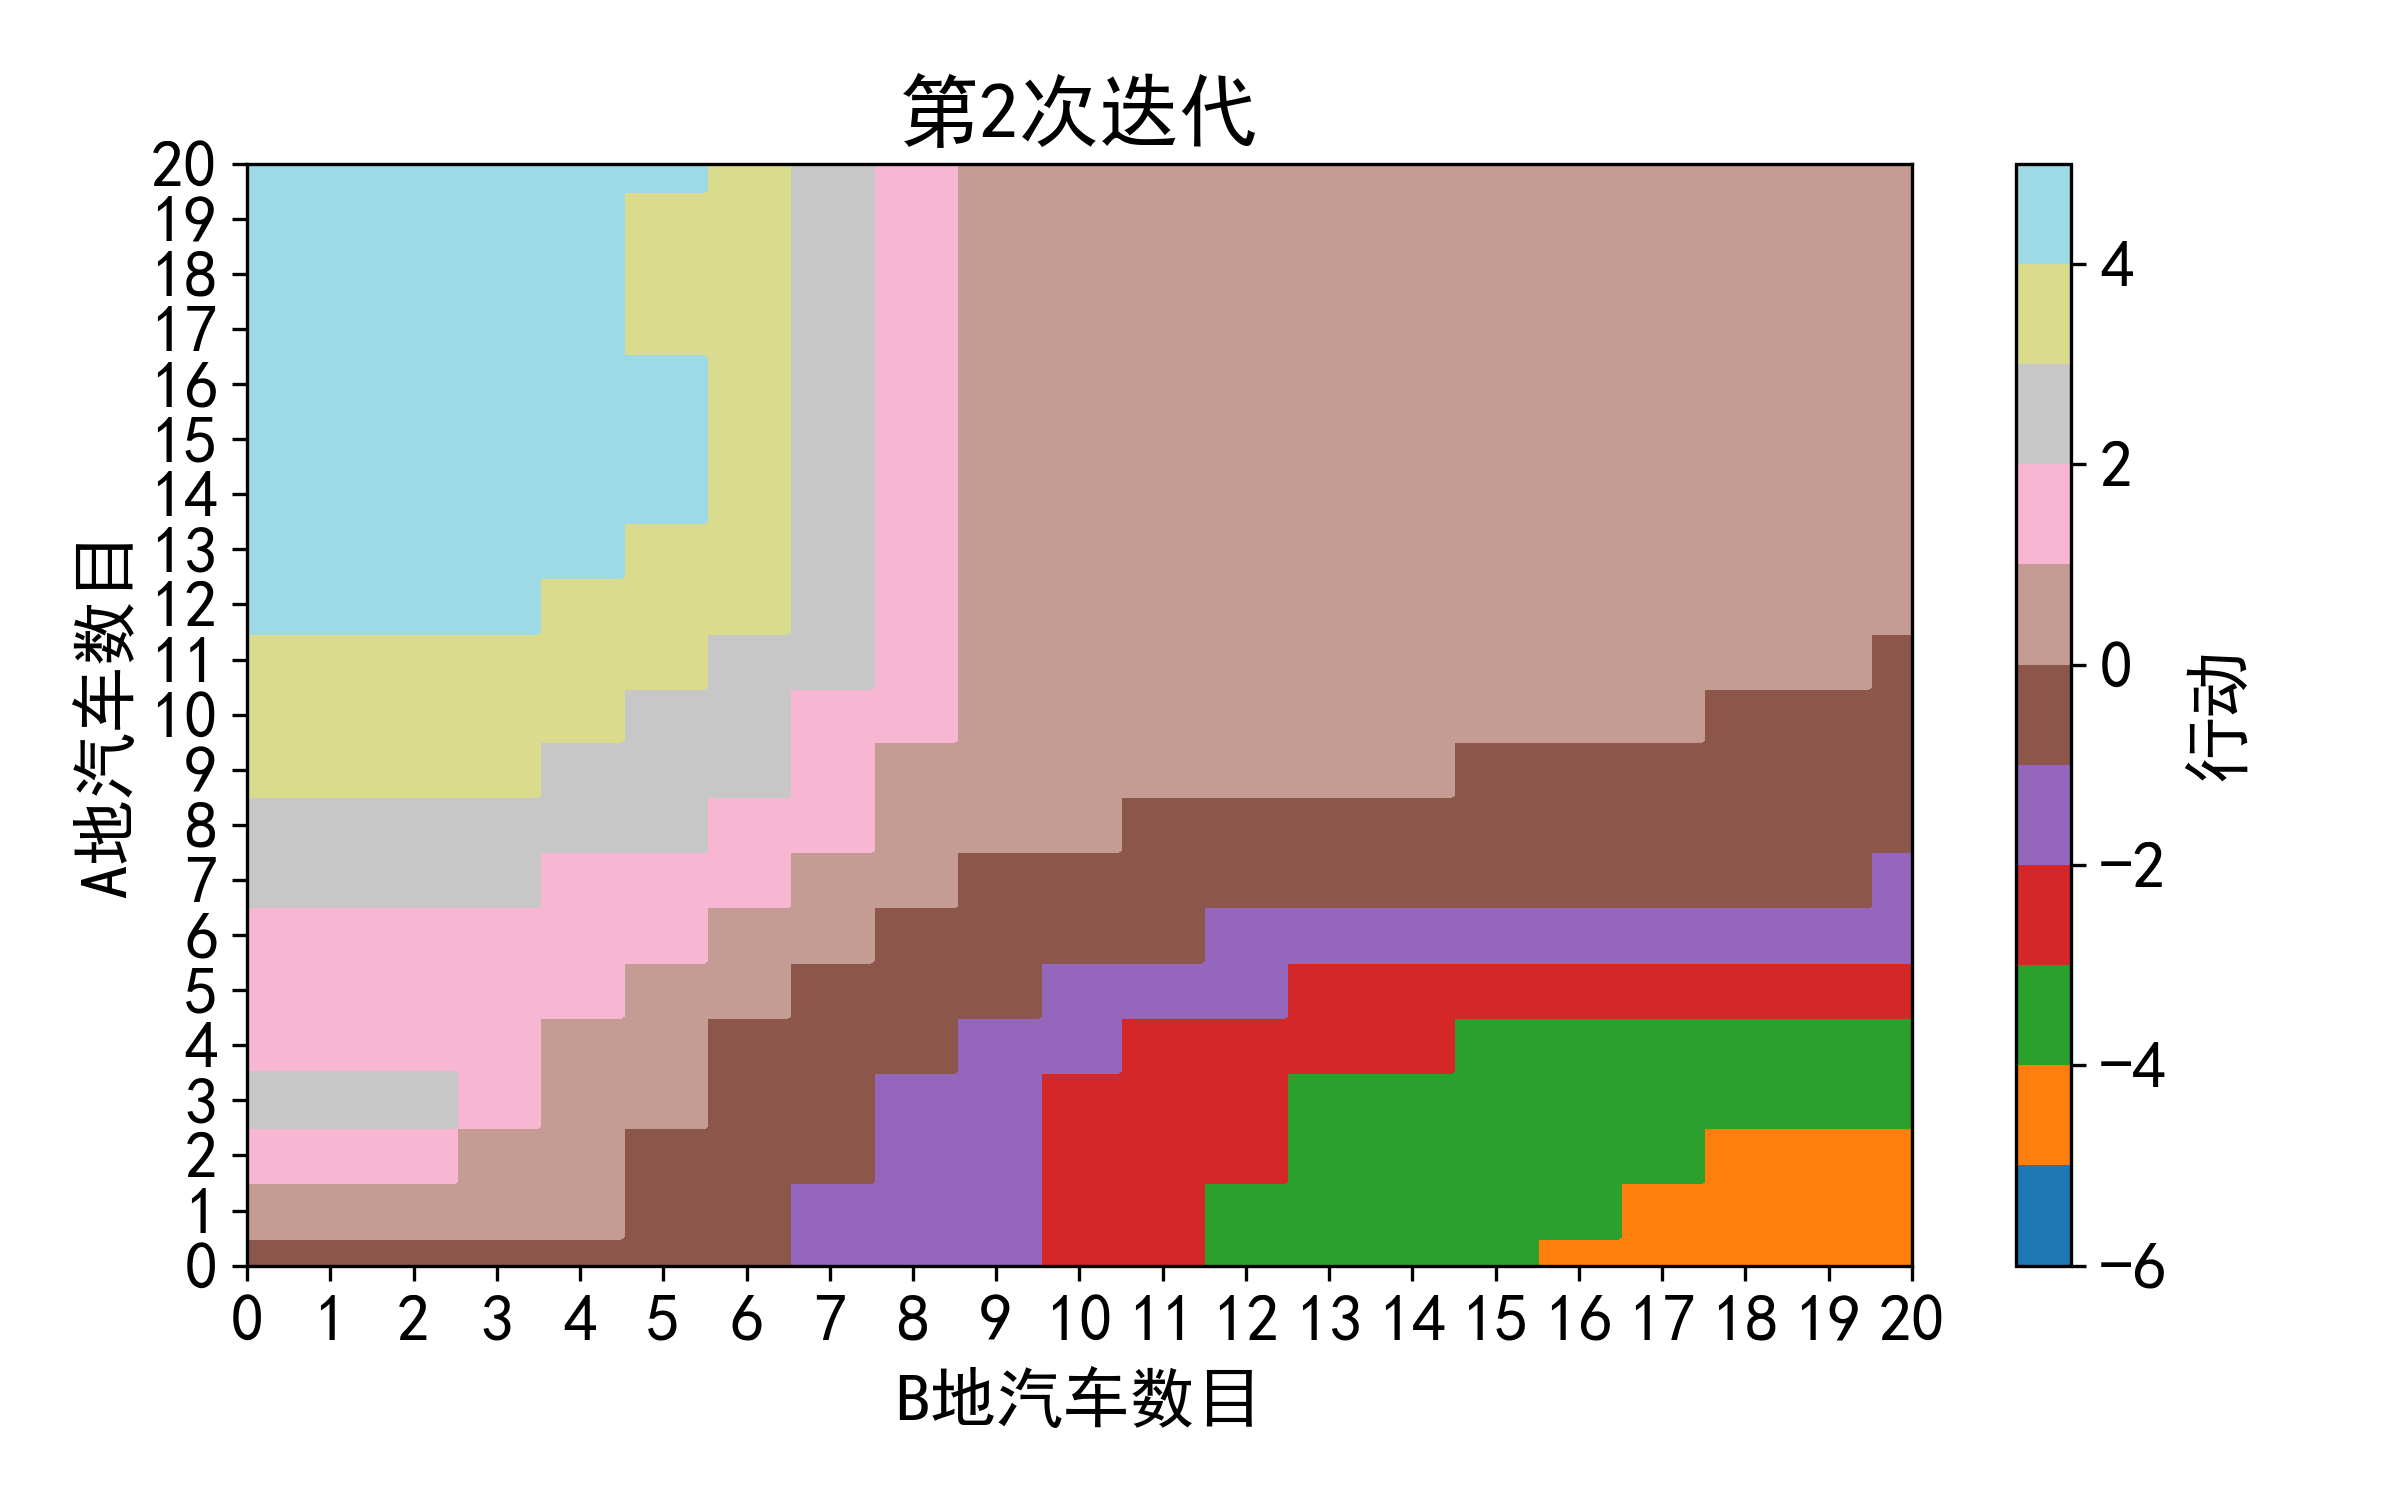
\includegraphics[scale=0.52]{080/080页练习4.7policy2.png}
            \end{minipage}
        }
    \end{figure}
    \clearpage
    \begin{figure}[htbp]
        \hspace{-0.5cm}
        \subfigure  % 子图的标题
        {
            % 如果一行放三个图改成0.3\linewidth即可
            \begin{minipage}[b]{.62\linewidth}
                \centering
                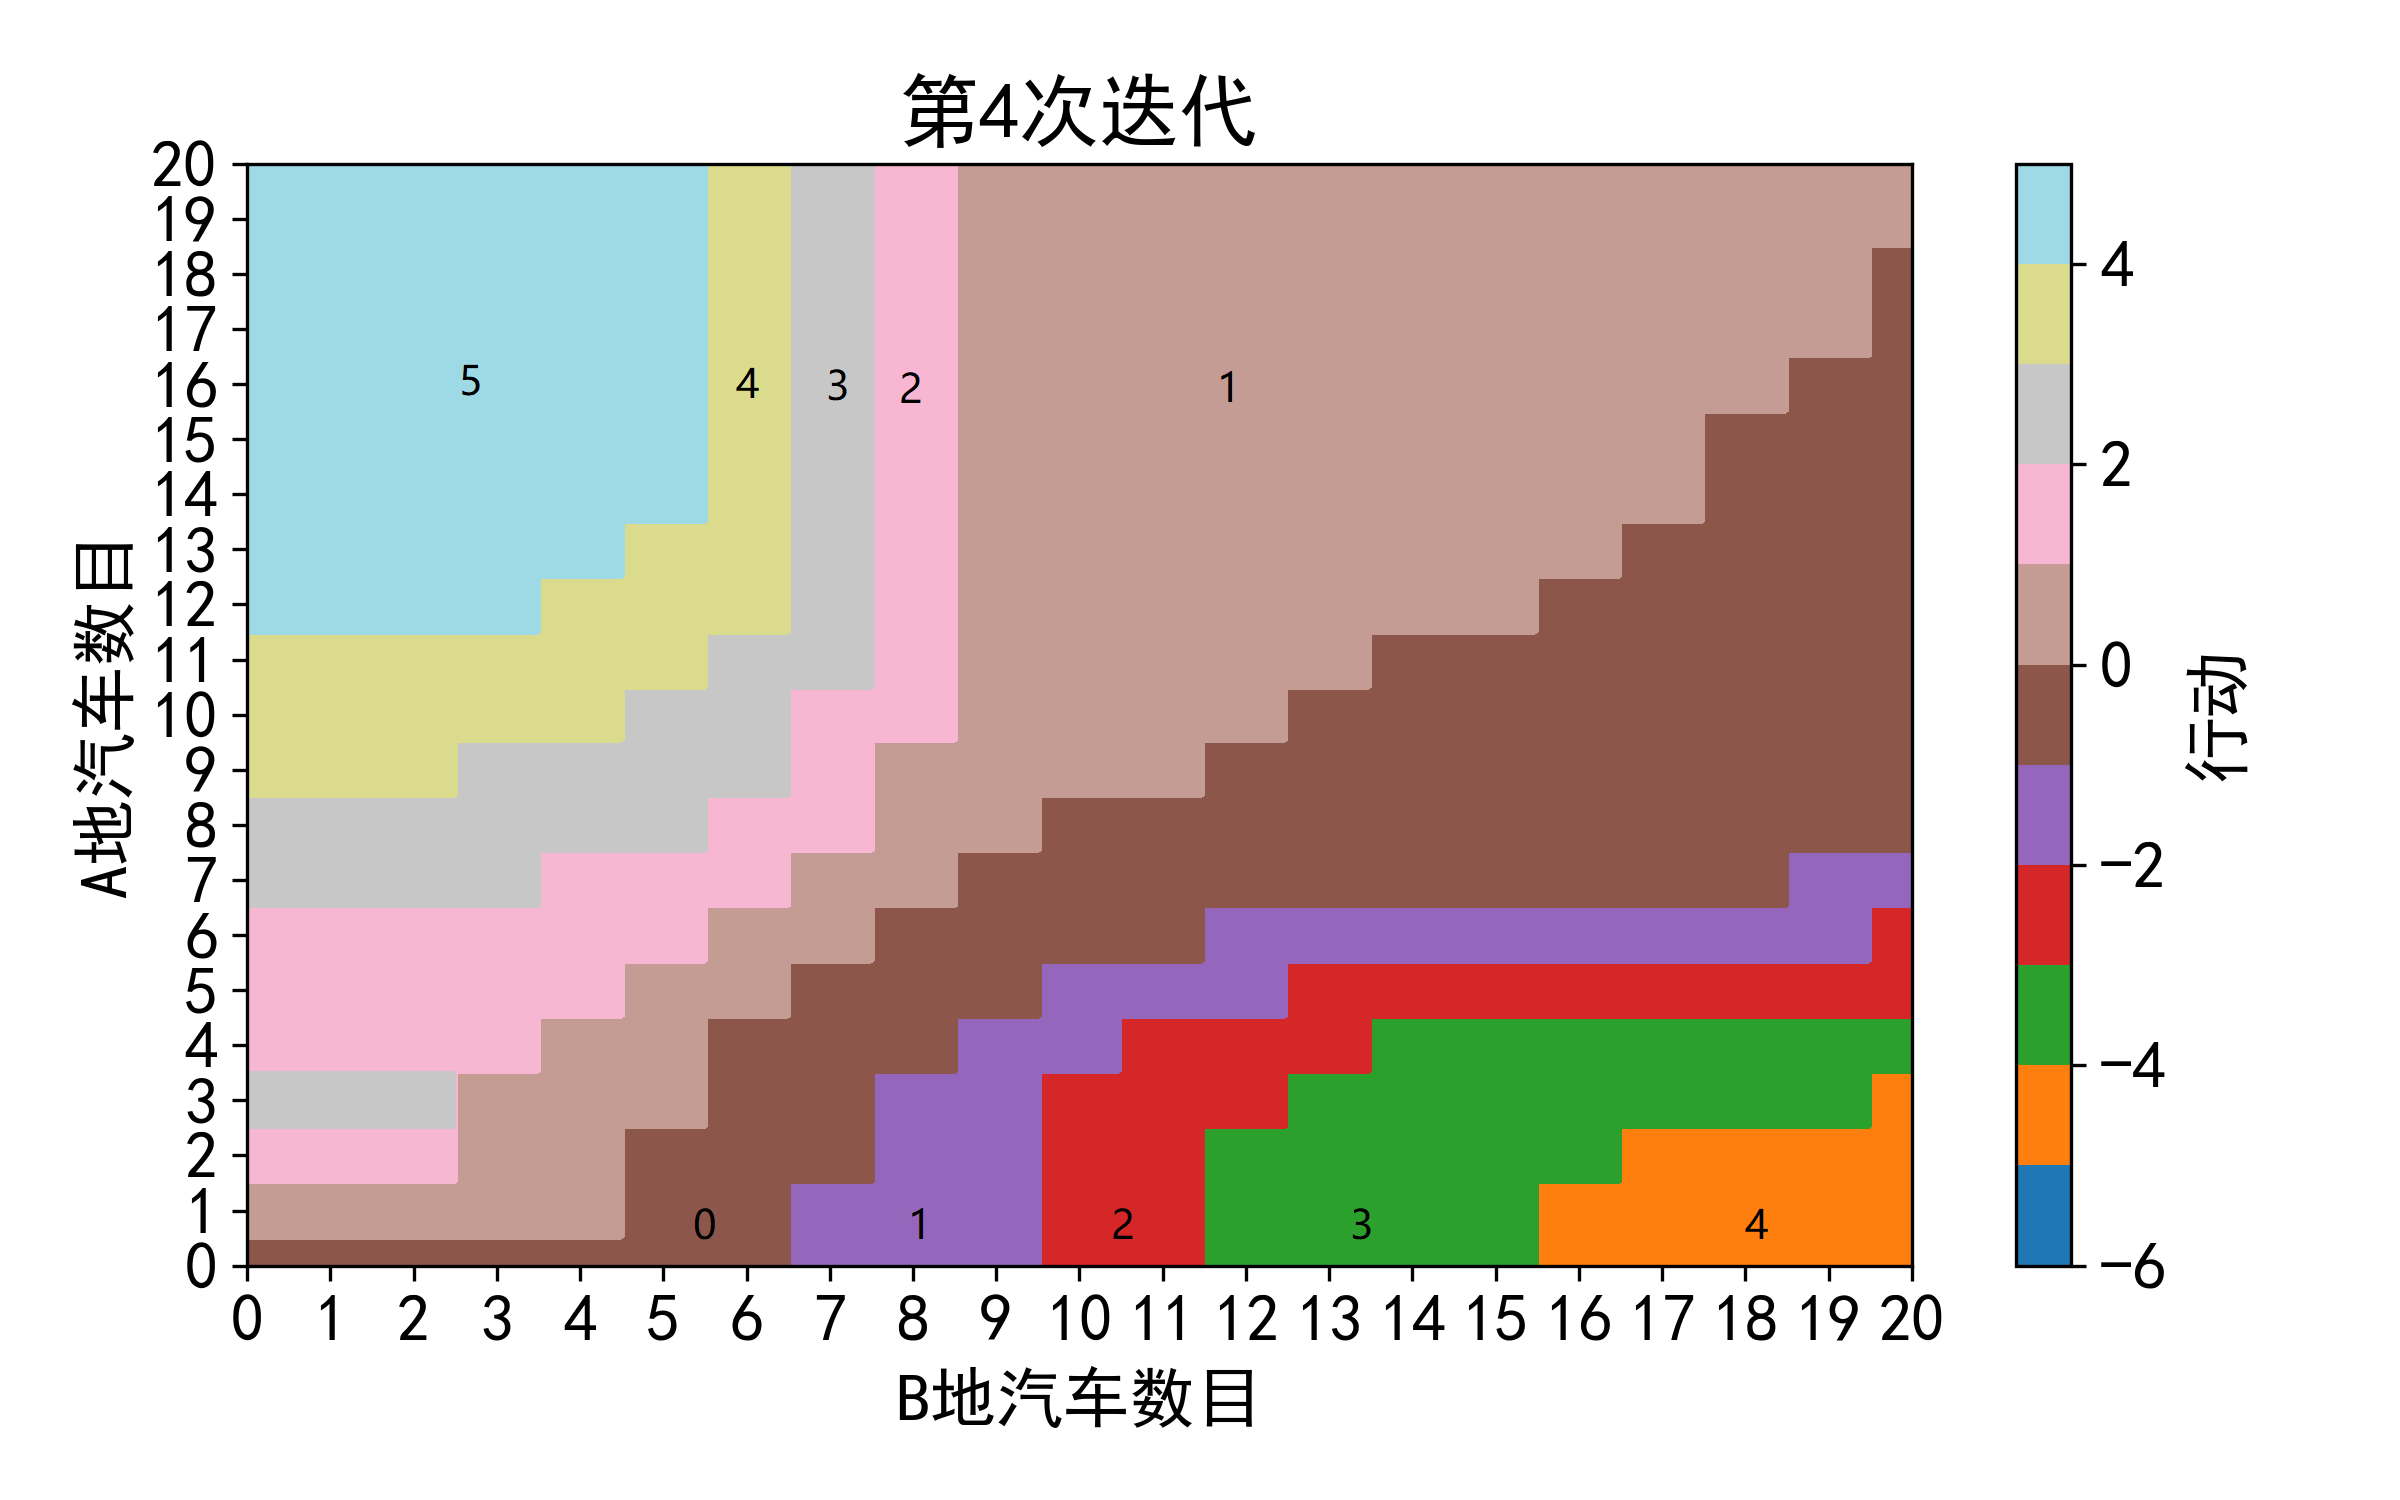
\includegraphics[scale=0.22]{080/080页练习4.7policy4.png}
            \end{minipage}
        }
        \subfigure
        {
            \begin{minipage}[b]{.2\linewidth}
                \centering
                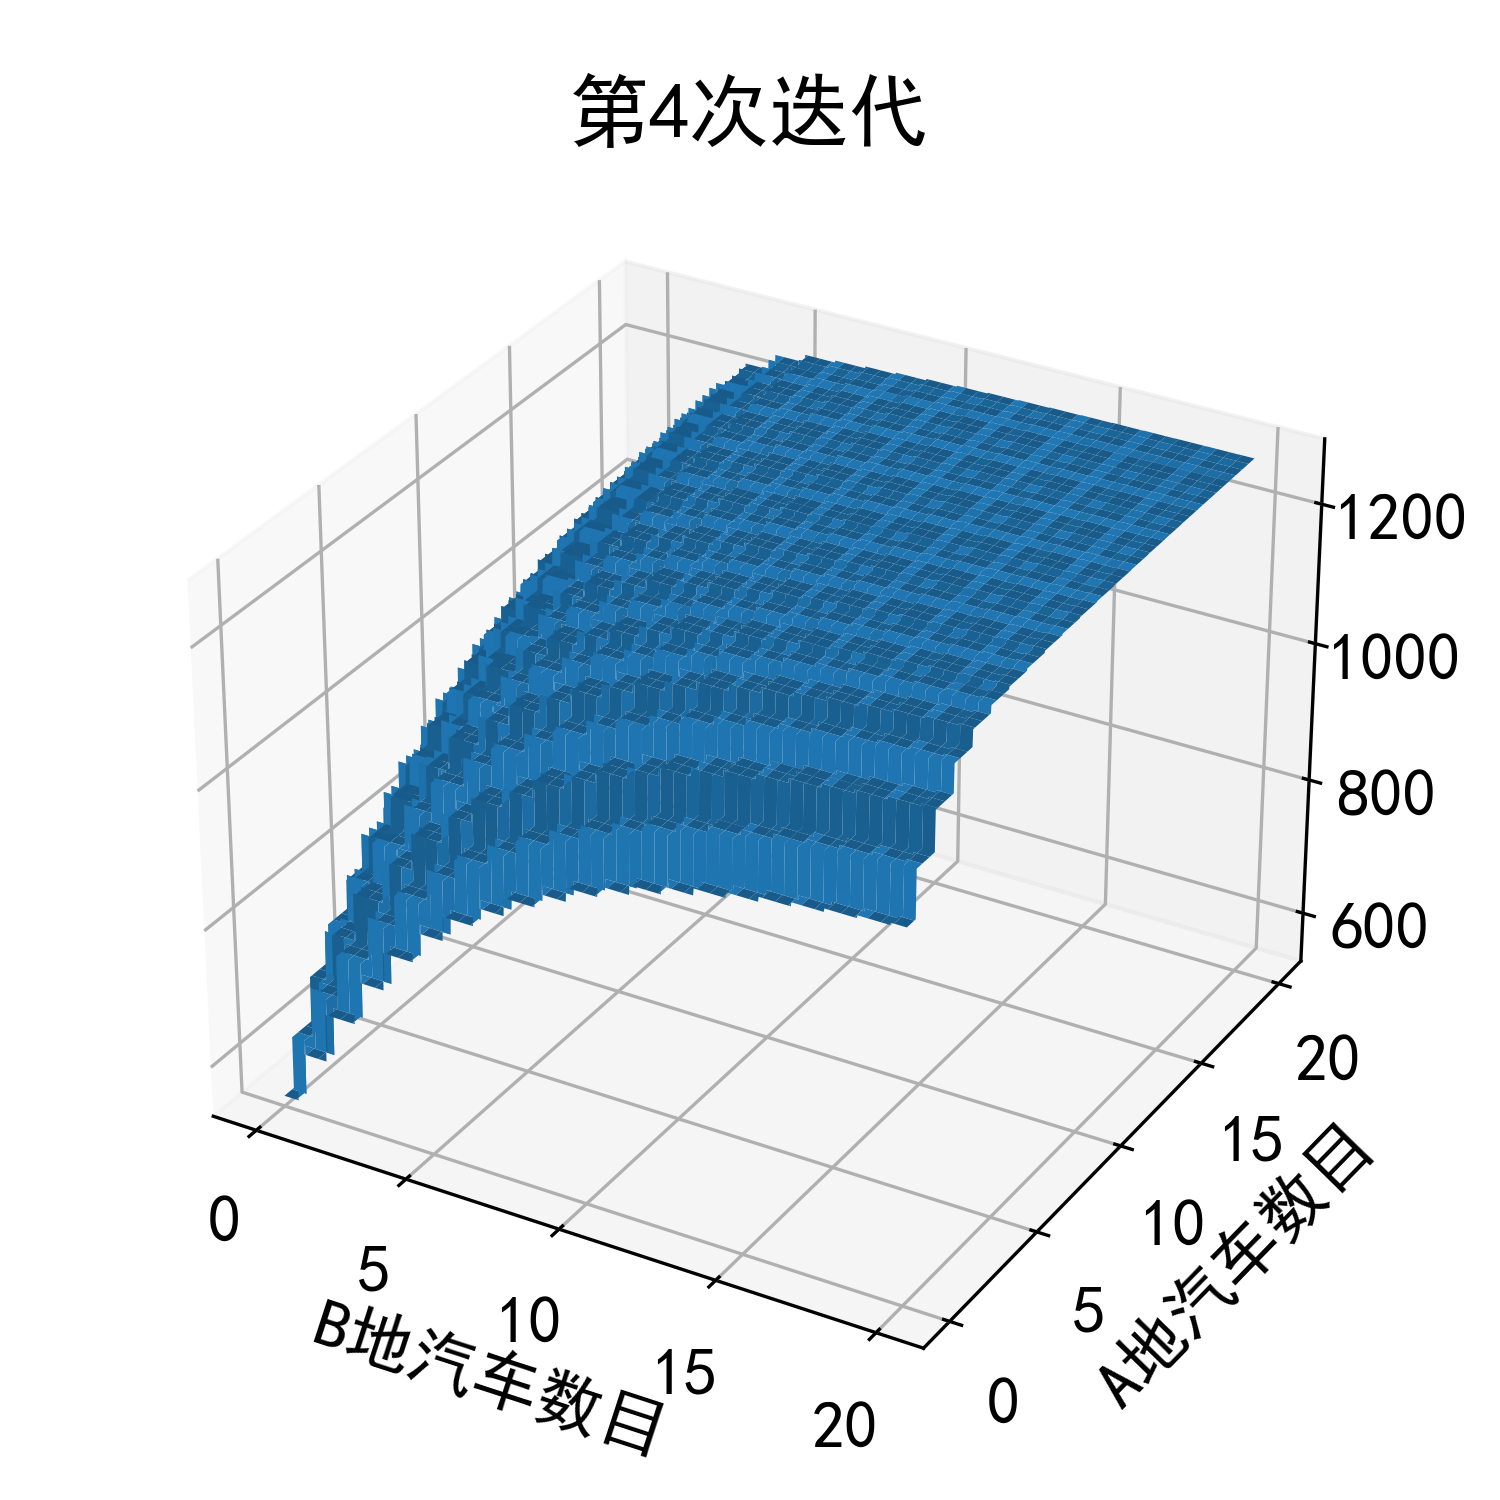
\includegraphics[scale=0.52]{080/080页练习4.7value4.png}
            \end{minipage}
        }
    \end{figure}
    \textbf{例4.2代码}:
    \begin{pythoncode}
import math
import numpy as np
import matplotlib as mpl
from tqdm import tqdm
import matplotlib.pyplot as plt

config = {  # matplotlib绘图配置
    "figure.figsize": (6, 6),  # 图像大小
    "font.size": 16, # 字号大小
    "font.sans-serif": ['SimHei'],   # 用黑体显示中文
    'axes.unicode_minus': False # 显示负号
}
plt.rcParams.update(config)

class Environment:
    def __init__(self, out_lambda, in_lambda, action_sign) -> None:
        self.out_lambda, self.in_lambda = out_lambda, in_lambda
        self.action_sign = action_sign  # 用于判断action前的符号
    
    def step(self, state, action, in_num, out_num):
        out_num = min(out_num, state)
        new_state = max(min(state - out_num + action * self.action_sign + in_num, 20), 0)
        reward = 10 * out_num
        return int(new_state), reward

    def poisson(self, x, lamb):
        return np.power(lamb, x) / math.factorial(x) * np.exp(-lamb)
    
    def get_prob(self, in_num, out_num):
        prob = self.poisson(in_num, self.in_lambda) * self.poisson(out_num, self.out_lambda)
        return prob


class Policy_iterate:
    def __init__(self, T=10, sample_num=5000, max_storageA=20, max_storageB=20, gamma=0.9) -> None:
        self.T = T
        self.sample_num = sample_num
        self.max_storageA, self.max_storageB = max_storageA, max_storageB
        self.gamma = gamma
        self.min_delta_value = 1e-3  # 价值函数改变量阈值
        self.envA = Environment(out_lambda=3, in_lambda=3, action_sign=-1)
        self.envB = Environment(out_lambda=4, in_lambda=2, action_sign=1)
    
    def work(self):
        self.policy = np.zeros((self.max_storageA+1, self.max_storageB+1))
        self.value = np.zeros((self.max_storageA+1, self.max_storageB+1))
        for _ in range(self.T):
            self.plot_policy(_)
            self.policy_estimate()
            delta_value, policy_stable = self.policy_improve()
            if delta_value <= self.min_delta_value:
                print(f"第{_}次迭代,状态价值变换{delta_value:.3f}小于阈值{self.min_delta_value:.3f},退出迭代")
                break
            if policy_stable is True:
                print(f"第{_}次迭代,策略已稳定,退出迭代")
                break

    def plot_policy(self, T):
        print(f"第{T}次迭代")
        print(self.policy)

        # 可视化策略
        plt.figure(figsize=(8, 5))
        x1, x2 = np.meshgrid(  # 创建离散网格点
            np.linspace(0, 20, 500),
            np.linspace(0, 20, 500)
        )
        # 计算高度值
        z = np.zeros_like(x1)
        for i in range(z.shape[0]):
            for j in range(z.shape[1]):
                z[i, j] = self.policy[round(x2[i, j]), round(x1[i, j])]
        # 设置等高线划分点,会根据情况绘制等高线,若没有相应的数据点,则不会进行绘制
        levelz = range(-6, 6)
        plt.contourf(x1, x2, z, levels=levelz, cmap='tab20')  # 向由等高线划分的区域填充颜色
        plt.colorbar(label='行动')  # 制作右侧颜色柱,表示每种颜色对应的值

        plt.xlabel('B地汽车数目')
        plt.ylabel('A地汽车数目')
        plt.xticks(range(0, 21))
        plt.yticks(range(0, 21))
        plt.grid(False)
        plt.title(f"第{T}次迭代")
        plt.tight_layout()
        plt.savefig(f"policy{T}.png", dpi=300)

        # 可视化状态价值
        fig = plt.figure(figsize=(5, 5))
        ax = fig.add_subplot(projection='3d')
        x1, x2 = np.meshgrid(  # 创建离散网格点
            np.linspace(0, 20, 1000),
            np.linspace(0, 20, 1000)
        )
        z = np.zeros_like(x1)
        for i in range(z.shape[0]):
            for j in range(z.shape[1]):
                z[i, j] = self.value[round(x2[i, j]), round(x1[i, j])]
        ax.plot_surface(x1, x2, z)
        ax.set_xlabel("B地汽车数目")
        ax.set_ylabel("A地汽车数目")
        plt.title(f"第{T}次迭代")
        plt.tight_layout()
        plt.savefig(f"value{T}.png", dpi=300)

        np.savetxt(f"policy{T}.txt", self.policy, fmt="%.0f")
        np.savetxt(f"value{T}.txt", self.value, fmt="%.2f")

    def calculate_value(self, stateA, stateB, action, value):
        new_value = 0
        for in_numA in range(6):
            for out_numA in range(6):
                probA = self.envA.get_prob(in_numA, out_numA)
                if probA < 0.0001:
                    continue
                for in_numB in range(6):
                    for out_numB in range(1, 7):
                        prob = probA * self.envB.get_prob(in_numB, out_numB)
                        new_stateA, rewardA = self.envA.step(stateA, action, in_numA, out_numA)
                        new_stateB, rewardB = self.envB.step(stateB, action, in_numB, out_numB)
                        reward = 10 * (rewardA + rewardB) - 2 * abs(action)
                        new_value += prob * (reward + self.gamma * value[new_stateA, new_stateB])
        return new_value

    def policy_estimate(self):
        min_delta_value = 1e-3
        T = 100
        for _ in range(T):
            value_backup = self.value.copy()
            delta_value = 0
            for stateA in range(self.max_storageA+1):
                for stateB in range(self.max_storageB+1):
                    old_value = self.value[stateA, stateB]
                    action = self.policy[stateA, stateB]
                    new_value = self.calculate_value(stateA, stateB, action, value_backup)
                    self.value[stateA, stateB] = new_value
                    delta_value = max(delta_value, abs(new_value - old_value))
            print(delta_value)
            if delta_value <= min_delta_value:
                break

    def policy_improve(self):
        delta_value, policy_stable = 0, True
        for stateA in range(self.max_storageA+1):
            for stateB in range(self.max_storageB+1):
                old_action = self.policy[stateA, stateB]
                max_value = 0
                for action in range(-5, 6):
                    if (action < 0 and stateB < -action) or (action > 0 and stateA < action):
                        continue
                    new_value = self.calculate_value(stateA, stateB, action, self.value)
                    if new_value > max_value:
                        max_value = new_value
                        self.policy[stateA, stateB] = action
                if old_action != self.policy[stateA, stateB]:
                    policy_stable = False
                delta_value = max(delta_value, abs(self.value[stateA, stateB] - max_value))
        return delta_value, policy_stable

if __name__ == '__main__':
    np.random.seed(42)
    agent = Policy_iterate()
    agent.work()
    \end{pythoncode}
    \textbf{练习4.7代码}:将\textbf{例4.2代码}中120行收益函数改为
    \begin{pythoncode}
    reward = -4 * (new_stateA > 10) - 4 * (new_stateB > 10)  # 额外停车费
    if action > 0:
        reward = 10 * (rewardA + rewardB) - 2 * (action - 1)
    else:
        reward = 10 * (rewardA + rewardB) + 2 * action
    \end{pythoncode}
\end{solution}
\end{document}